\documentclass[12pt]{amsart}
\usepackage{amsmath,amsthm,amssymb,amsfonts,enumerate,mymath,tikz-cd,fancyhdr}
\openup 5pt
\author{Blake Farman\\University of South Carolina}
\title{Math 111: Exam 02 Solutions}
\date{June 7, 2013}
\pdfpagewidth 8.5in
\pdfpageheight 11in
\usepackage[margin=1in]{geometry}

\renewcommand{\qedsymbol}{}

\begin{document}
\maketitle

\begin{center}
  \fbox{\fbox{\parbox{5.5in}{\centering
        Answer the questions in the spaces provided on the
        question sheets and turn them in at the end of the class period. 
        Unless otherwise stated, all supporting work is required.}}}
\end{center}

\vspace{0.2in}
\makebox[\textwidth]{Name:\enspace\hrulefill}
\vspace{0.2in}

\theoremstyle{plain}
\newtheorem{thm}{}
\newtheorem{lem}{Lemma}
\theoremstyle{definition}
\newtheorem{defn}{Definition}

\section{Definitions}
\begin{thm}[4 Points]\label{ex1}
  \begin{enumerate}[(a)]
  \item
    State the Point-Slope form of a line passing through the point $(x_1, y_1)$ with slope $m$.
  \item
    State the Slope-Intercept form of a line with slope $m$ and $y$-intercept $b$.
  \end{enumerate}
  
  \begin{proof}[Solution]
    \begin{enumerate}[(a)]
    \item
      The Point-Slope form of a line passing through the point $(x_1, y_1)$ with slope $m$ is
      $$y - y_1 = m(x - x_1).$$
    \item
      The Slope-Intercept form of a line with slope $m$ and $y$-intercept $b$ is
      $$y = mx + b.$$
    \end{enumerate}
  \end{proof}
\end{thm}

\begin{thm}[6 Points]\label{ex2}
  Let $f(x)$ be a function.
  State the average rate of change of $f$ between $x = a$ and $x = b$.
  
  \begin{proof}[Solution]
    The average rate of change of $f$ between $x = a$ and $x = b$ is
    $$\frac{f(b) - f(a)}{b - a}\ \text{or}\ \frac{f(a) - f(b)}{a - b}.$$
  \end{proof}
\end{thm}

\begin{thm}[5 Points]\label{ex3}
  State the growth rate formula for a function $f(x)$.
  
  \begin{proof}[Solution]
    The growth rate formula for a function $f(x)$ is 
    $$r = \frac{f(x + 1) - f(x)}{f(x)}.$$
  \end{proof}
\end{thm}

\begin{thm}[3 Points]\label{ex4}
  \begin{enumerate}[(a)]
  \item
    State the general form of an exponential function.
    \item
      When does such a function model exponential growth?
    \item
      When does such a function model exponential decay?
  \end{enumerate}
  
  \begin{proof}[Solution]
    \begin{enumerate}[(a)]
    \item
      The general form of an exponential function is $$f(t) = Ca^t.$$
    \item
      The function $f$ models exponential growth when $a > 1$.
    \item
      The function $f$ models exponential decay when $0 < a < 1$.
    \end{enumerate}
  \end{proof}
\end{thm}

\begin{thm}[2 Points]
  Consider the two lines $f(x) = m_1x + b_2$ an $g(x) = m_2x + b_2$.
  \begin{enumerate}[(a)]
  \item
    When are $f$ and $g$ parallell
  \item
    When are $f$ and $g$ perpendicular?
  \end{enumerate}

  \begin{proof}[Solution]
    \begin{enumerate}[(a)]
    \item
      The lines $f$ and $g$ are parallel whenever $m_1 = m_2$.
    \item
      The lines $f$ and $g$ are perpendicular whenever any of the following three equivalent conditions hold,
      \begin{enumerate}[(i)]
        \item
          $m_1m_2 = -1$,
        \item
          $m_1 = -\frac{1}{m_2}$, or
        \item
          $m_2 = -\frac{1}{m_1}$.
      \end{enumerate}
    \end{enumerate}
  \end{proof}
\end{thm}


\section{Problems}

\begin{thm}[16 Points]\label{ex5}
  In the following problems, use the given information to find the equation of the line in slope-intercept form.
  \begin{enumerate}[(a)]
  \item
    The line passing through the points $(2,5)$ and $(4,13)$.
  \item
    The line passing through the point $(-3, 3)$ and parallel to the line $2y - 4x = 20$.
  \item
    The line passing through the origin (that is, the point $(0,0)$) and perpendicular to the line $2y - 4x = 20$.
  \end{enumerate}
  \begin{proof}[Solution]
    \begin{enumerate}[(a)]
    \item
      First we calculate the slope of the line, $m$,
      $$m = \frac{13 - 5}{4 - 2} = \frac{8}{2} = 4\ \text{or}\ m = \frac{5 - 13}{2 - 4} = \frac{-7}{-2} = 4.$$
      Then we can form either of two lines in Point-Slope form,
      $$y - 13 = 4(x - 4)\ \text{or}\ y - 5 = 4(x - 2).$$
      For the first one, we can put it into Slope-Intercept form by distributing on the right-hand side and adding 13 to both sides, which gives
      $$y = 4x - 16 + 13 = 4x - 3.$$
      For the second, we distribute on the right-hand side and add 5 to both sides to obtain
      $$y = 4x - 8 + 5 = 4x - 3.$$

      As a second alternative, you could also compute the $y$-intercept using either of the points $(2,5)$ and $(4,13)$.
      Since we know the line passes through the point $(2,5)$, if we assume the line has the form $y = mx + b$, we have the equation
      $$5 = 4(2) + b,$$
      which gives us $$b = 5 - 8 = -3.$$
      Similarly, if we use the point $(4,13)$ we have the equation
      $$13 = 4(4) + b$$
      and this gives $$b = 13 - 16 = -3.$$
    \item
      Since we know that two lines are parallel whenever they have the same slope, we start start by determining the slope of the line $2y - 4x = 20$.
      To do this we add $4x$ to both sides to get 
      $$2y = 4x + 20$$
      and divide both sides by $2$ to get
      $$y = 2x + 10.$$
      Hence our slope will be $m = 2$ and the Point-Slope form of the line passing through $(-3,3)$ is 
      $$y - 3 = 2(x - (-3)) = 2(x + 3).$$
      To put this equation into Slope-Intercept form we distribute on the right-hand side and add $3$ to both sides, which gives
      $$y = 2x + 6 + 3 = 2x + 9.$$
    \item
      Since we've already computed the slope, $m = 2$, of the line $2y - 4x = 20$, we use the fact that the slope of a perpendicular line must be $-\frac{1}{m} = -\frac{1}{2}$.
      Moreover we know that this line passes through the origin, and so our $y$-intercept is $b = 0$.
      Therefore the line perpendicular to $2y - 4x = 20$ that passes through the origin is
      $$y = -\frac{1}{2}x.$$
    \end{enumerate}
  \end{proof}
\end{thm}


\begin{thm}[16 Points]\label{ex10}
  Consider the two lines $f(x) = 4x + 3$ and $g(x) = x + 12$.
  Find the point (that is, the $(x,y)$ pair) where these two lines intersect.
  
  \begin{proof}[Solution]
    To find the point where these two lines intersect we find the $x$-coordinate of the intersection by solving the equation
    $$4x + 3 = x + 12$$
    for $x$.
    Subtracting $x$ from both sides we have
    $$4x - x + 3 = 3x + 3 = 12.$$
    We then subtract $3$ from both sides to get 
    $$3x = 9$$
    and divide both sides by $3$ to arrive at 
    $$x = 3.$$
    To find the $y$-coordinate, we can evaluate either line at $x = 3$.
    The easier of the two to compute is 
    $$g(3) = 3 + 12 = 15.$$
    Note that we could also compute
    $$f(3) = 4(3) + 3 = 12 + 3 = 15$$
    and arrive at the same answer.
    Therefore the point where these two lines intersect is $(3, 15)$.
  \end{proof}
\end{thm}



\begin{thm}[16 Points]\label{ex9}
  Let $f(x) = x^2$.
  \begin{enumerate}[(a)]
  \item
    Compute the average rate of change for $f$ between $x = 2$ and $x = 5$.
  \item
    Give the Point-Slope form of a line that passes through $(2, f(2))$ and $(5, f(5))$.
  \item
    Give the Slope-Intercept form of a line that passes through $(2, f(2))$ and $(5, f(5))$.
  \end{enumerate}
  
  \begin{proof}[Solution]
    \begin{enumerate}[(a)]
    \item
      The average rate of change of $f$ between $x = 2$ and $x = 5$ is given by
      $$\frac{f(5) - f(2)}{5 - 2} = \frac{25 - 4}{3} = \frac{21}{3} = 7$$
      or
      $$\frac{f(2) - f(5)}{2 - 5} = \frac{4 - 25}{-3} = \frac{-21}{-3} = 7.$$
    \item
      The average rate of change computed in part (a) is the slope of the line passing through $(2, f(2)) = (2,4)$ and $(5, f(5)) = (5, 25)$, so the Point-Slope form is given by either of the following equations
      \begin{enumerate}[(i)]
      \item
        $y - 4 = 7(x - 2)$, or
      \item
        $y - 25 = 7(x - 5)$.
      \end{enumerate}
    \item
      We may use either equation above to find the Slope-Intercept form of the line.  
      Using the first we distribute on the right-hand side and add 4 to both sides to obtain
      $$y = 7x - 14 + 4 = 7x - 10.$$
      Using the second, we distribute on the right hand side and add 25 to both sides to get
      $$y = 7x - 35 + 25 = 7x - 10.$$
    \end{enumerate}
  \end{proof}
\end{thm}

\begin{thm}[16 Points]\label{ex7}
  Alice is hosting an event.  She is renting a facility, which costs $\$300$, and providing refreshments, which cost $\$4$ per guest.
  \begin{enumerate}[(a)]
  \item
    Find a function, $C$, that models the total cost of the event if $x$ people attend.
  \item
    Sketch a graph of $C$.
  \item
    Evaluate $C(10)$ and $C(15)$.  What do these numbers represent?
  \item
    If the total cost for the event was $400$, how many people attended?
  \end{enumerate}
  
  \begin{proof}[Solution]
    \begin{enumerate}[(a)]
    \item
      Since the $\$300$ to rent the facility is paid even if no guests attend, this is our initial value for the cost function.
      We know that each additional guest increases the cost of the event by $\$4$, so our cost function is
      $$C(x) = 4x + 300.$$
    \item
      Below is a plot of the function.  
      Note that it does not include portions where $x < 0$ since there is no reasonable meaning for a negative number of guests.
      \begin{center}
        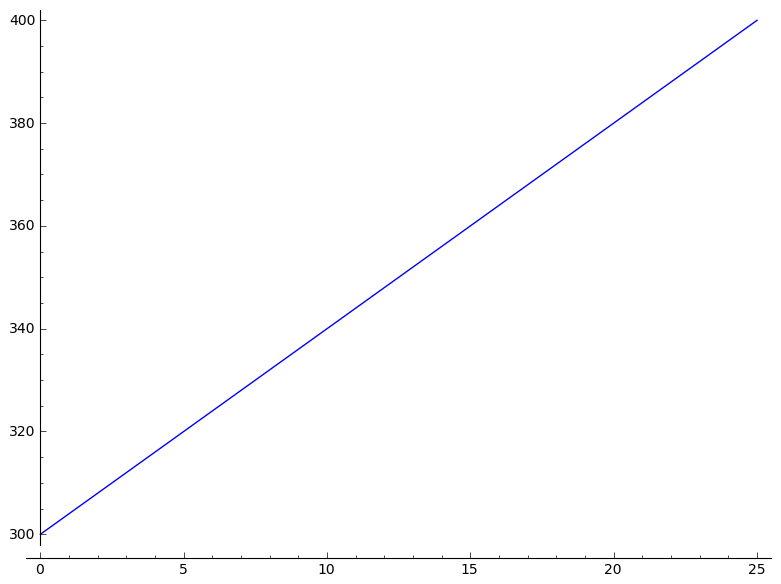
\includegraphics[scale=0.5]{plot.png}
      \end{center}
    \item
      When $x = 10$ we have
      $$C(10) = 4(10) + 300 = 40 + 300 = 340.$$
      This models the cost of the event if $10$ guests attend.
      When $x = 15$ we have
      $$C(15) = 4(15) + 300 = 60 + 300 = 360.$$
      This models the cost of the event if $15$ guests attend.
    \item
      If the cost of the event is $\$400$, then we know 
      $$400 = 4x + 300.$$
      Subtracting 300 from both sides we have
      $4x = 400 - 300 = 100$
      and dividing both sides by $100$ gives us
      $x = 25$.
      Therefore if the cost of the event is $\$400$, $25$ guests attended.
    \end{enumerate}
  \end{proof}
\end{thm}



\begin{thm}[16 Points]
  A population of size $25$ grows by $20\%$ every day.
  \begin{enumerate}[(a)]
  \item
    Give the growth factor for this population.
  \item
    Give an exponential model for the size of the population after $t$ days.
  \item
    Determine the size of the population after 2 days.  [Hint: Express the growth factor as a ratio, rather than a decimal, and this will be easy to compute.]
  \end{enumerate}
  
  \begin{proof}[Solution]
    \begin{enumerate}[(a)]
    \item
      We are given the growth rate, $r = 20\% = \frac{20}{100} = {1}{5}$, so to find the growth factor we use the formula
      $$a = 1 + r = 1 + \frac{1}{5} = \frac{5}{5} + \frac{1}{5} = \frac{6}{5}.$$
    \item
      We are given the initial population, $25$, and we have calculated the growth factor $a = \frac{6}{5}$, so our exponential model is
      $$P(t) = 25\left(\frac{6}{5}\right)^t.$$
      Note that our $t$ value here is measured in days.
    \item
      After two days, our population is given by computing $P(2)$.
      Therefore the population is
      $$P\left(2\right) = 25 \cdot \left(\frac{6}{5}\right)^2 = 25 \cdot \frac{6^2}{5^2} = 25 \cdot \frac{36}{25} = 36.$$
    \end{enumerate}
  \end{proof}
\end{thm}

\begin{thm}[Bonus - 10 Points]\label{bonus}
  Let $f\left(x\right) = m_1x + b_1$ and $g\left(x\right) = m_2x + b_2$.
  Using $f$ and $g$, derive the general formula for the intersection of two lines.
  Use this to explain why two parallel lines never intersect.
  
  \begin{proof}[Solution]
    To compute the point of intersection for two lines we first compute the $x$-coordinate by solving the equation
    $$m_1x + b_1 = m_2x + b_2$$
    for $x$.
    Subtracting $m_2x$ from both sides we get the equation
    $$m_1x - m_2x + b_1 = (m_1 - m_2)x + b_1 = b_2.$$
    Subtracting $b_1$ from both sides gives us
    $$(m_1 - m_2)x = b_2 - b_1.$$
    Now, to solve for $x$ we must divide both sides of the equation by $m_1 - m_2$, which means that $m_1 - m_2 \neq 0$ must hold.
    This is exactly the condition that $m_1 \neq m_2$, i.e. these lines must {\it not} be parallel, which shows that two parallel lines never intersect (except, of course, in the case where $f$ and $g$ are exactly the same line, in which case they 'intersect' at value of $x$).
    If we assume that $f$ and $g$ are not parallel then we know that $m_1 - m_2 \neq 0$ and so 
    $$x = \frac{b_2 - b_1}{m_1 - m_2}.$$

    To find the $y$-coordinate of the point of intersection, we evaluate either line at the $x$ value above.
    This gives
    \begin{eqnarray*}
      f\left(\frac{b_2 - b_1}{m_1 - m_2}\right) &=& m_1\left(\frac{b_2 - b_1}{m_1 - m_2}\right) + b_1\\
      &=& \frac{m_1b_2 - m_1b_1}{m_1 - m_2} + b_1\frac{m_1 - m_2}{m_1 - m_2}\\
      &=& \frac{m_1b_2 - m_1b_1 + m_1b_1 - m_2b_1}{m_1 - m_2}\\
      &=& \frac{m_1b_2 - m_2b_1}{m_1 - m_2}.
    \end{eqnarray*}
    Therefore the point of intersection for any two lines is given by
    $$\left(\frac{b_2 - b_1}{m_1 - m_2}, \frac{m_1b_2 - m_2b_1}{m_1 - m_2}\right).$$
  \end{proof}
\end{thm}
\end{document}
